\documentclass[t, final]{beamer}

%
% Configure beamer
\usetheme{MRCBSU}
\usefonttheme{default}
\beamertemplatenavigationsymbolsempty
\usepackage[orientation=portrait, size=a0, scale=1]{beamerposter}

%
% blindtext used to insert dummy text
\usepackage[english]{babel}
\usepackage{blindtext}

%
% As close to Arial as we can easily get
\usepackage{helvet}
\renewcommand{\familydefault}{\sfdefault}

%
% Set up biblatex
\usepackage{csquotes}
\usepackage[
  doi=false,
  isbn=false,
  url=false,
  sorting=none,
  style=authoryear,
  %natbib,
  %bibstyle=numeric,
  %citestyle=reading,
  backend=biber]{biblatex}
%
% We specify the database.
\addbibresource{Clusternomics.bib}
\DeclareCiteCommand{\citejournal}
  {\usebibmacro{prenote}}
  {\usebibmacro{citeindex}%
   \usebibmacro{cite}
   \usebibmacro{journal}}
  {\multicitedelim}
  {\usebibmacro{postnote}}


\begin{document}
\begin{frame}{}

%
% Headers
\begin{block}{
  \vspace{24pt}

  
\includegraphics[height=150pt]{Figures/BSU}
  % \hspace{30pt}
  \hfill
  
\includegraphics[height=150pt]{Figures/UniCam}

  \vspace{24pt}
}
  \vspace{24pt}

  \begin{center}
    \fontsize{82pt}{82pt}\selectfont \textcolor{mrcblue}{\textbf{Clusternomics: integrating heterogeneous data}}
  \end{center}

  \vspace{24pt}

  %
  % Authors
  \fontsize{36pt}{36pt}\selectfont
  \textcolor{mrcblue}{
    Evelina Gabasova,
    John Reid,
    Lorenz Wernisch
    % \hspace{30pt}
    \hfill
    MRC Biostatistics Unit,
    %Cambridge Biomedical Campus,
    Cambridge,
    CB2 0SR,
    United Kingdom}
\end{block}


%
% Change block colours and font sizes...
\setbeamercolor{block title}{bg=white, fg=mrcblue}
\setbeamercolor{block body}{bg=white, fg=black}


%
% Columns
\begin{columns}[t]
\begin{column}{.32\linewidth}
\begin{block}{Typical cancer data}
  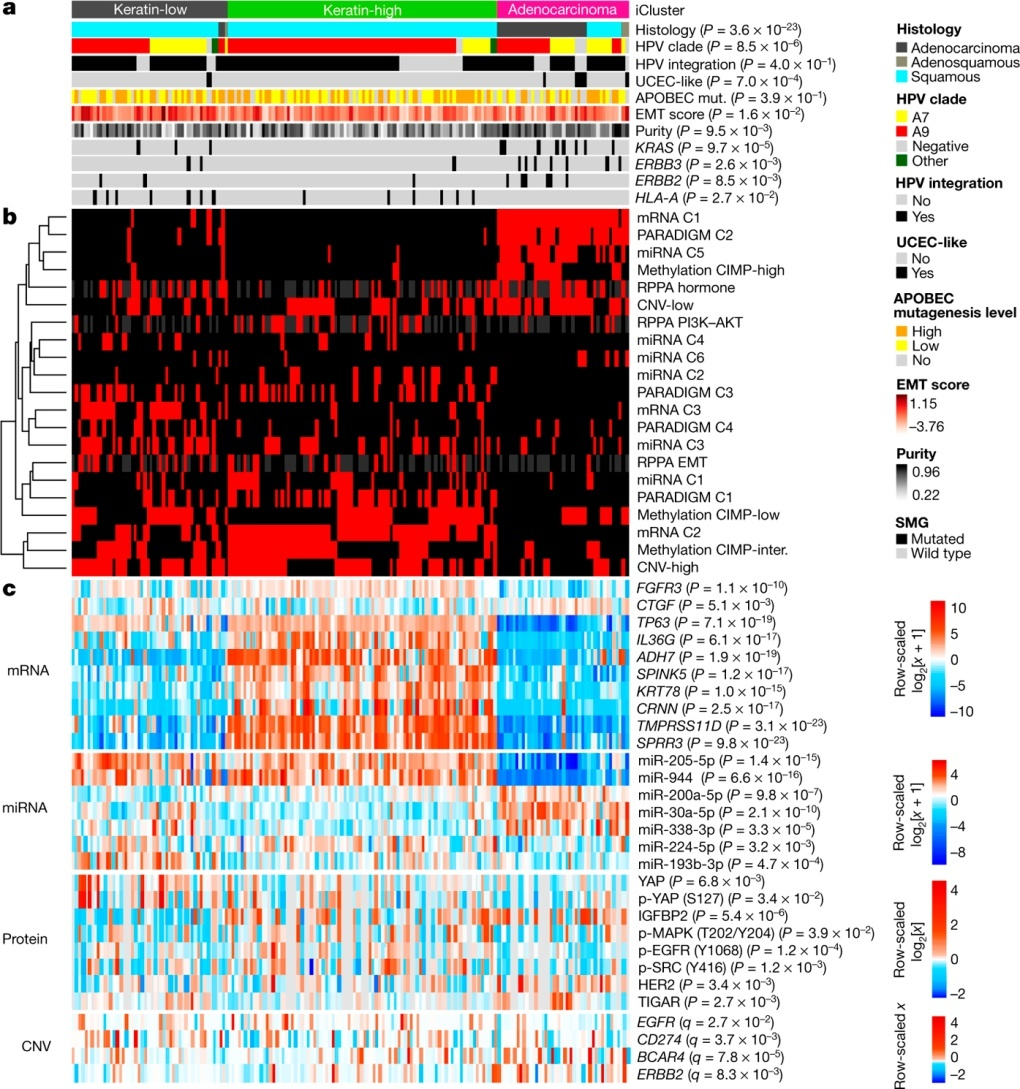
\includegraphics[width=\textwidth]{Figures/cervical-clusters}
  {\small \citejournal{the_cancer_genome_atlas_research_network_integrated_2017}}

  \begin{itemize}
    \item 178 cervical cancer samples
    \item Several data contexts
      \begin{itemize}
        \item[--] Varying cluster structure
        \item[--] Different views of biology
        \item[--] Not comparable
      \end{itemize}
    \item Heterogeneous disease
    \item Subtype identification
      \begin{itemize}
        \item[--] Disease understanding
        \item[--] Clinical significance
      \end{itemize}
    \item Noisy data
    \item Natural to cluster samples
  \end{itemize}
\end{block}

\begin{block}{Prior work}
  Bayesian consensus clustering (BCC): \\
  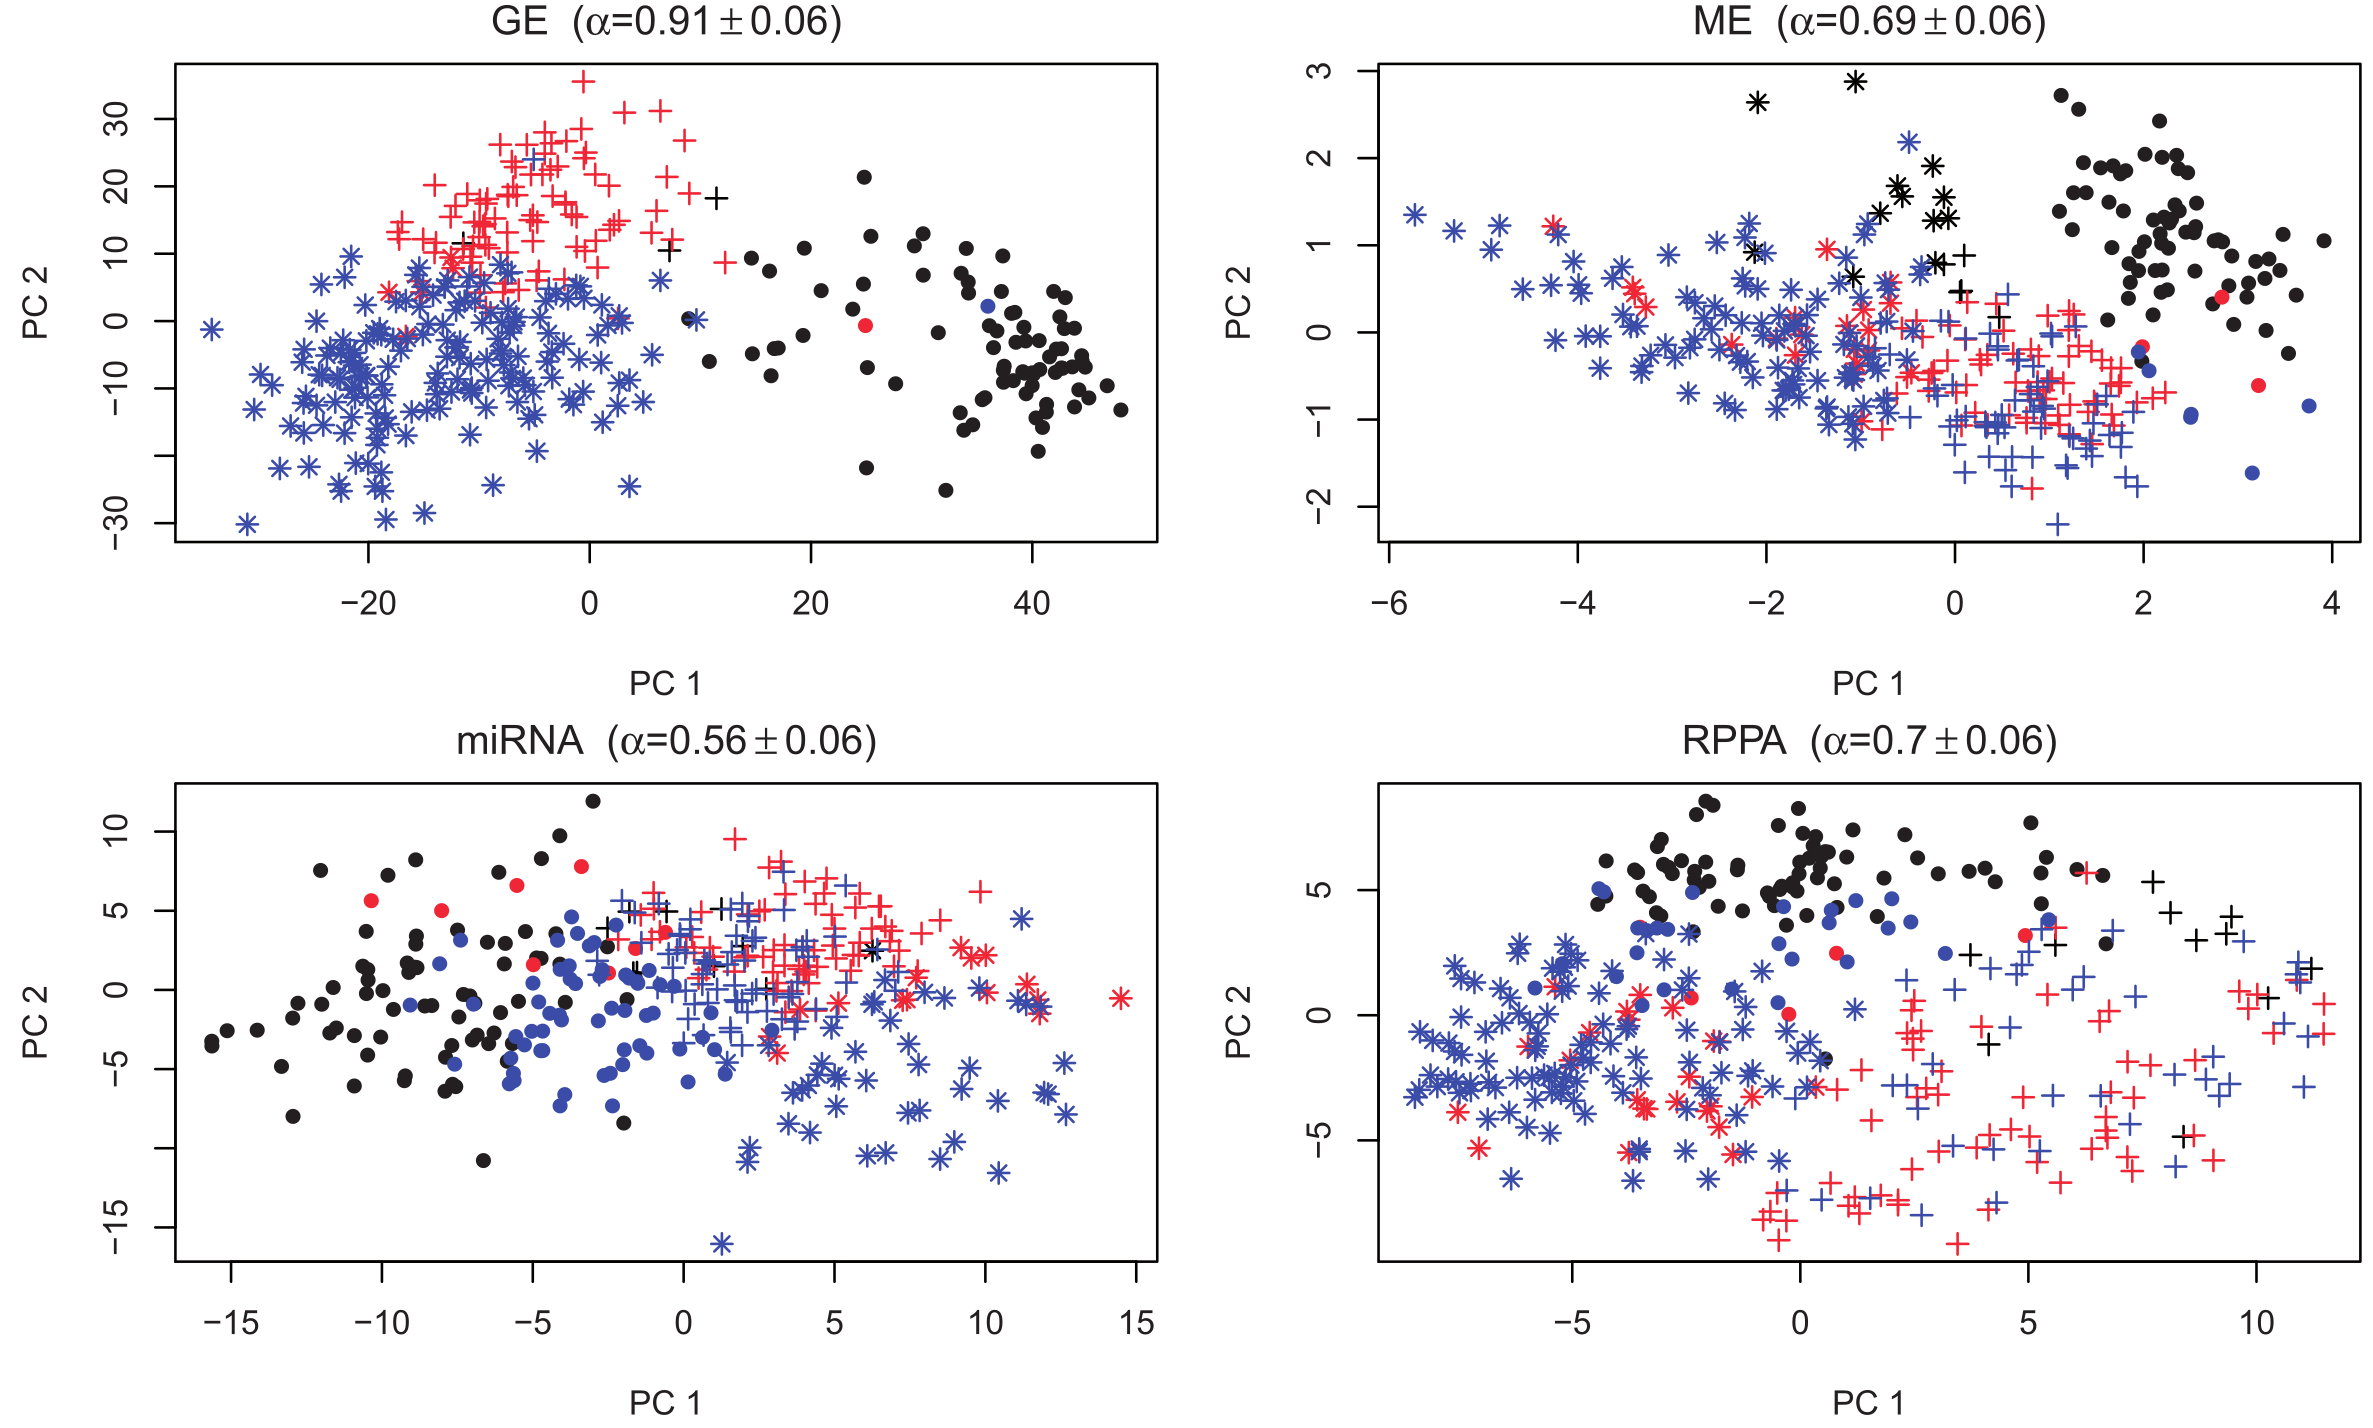
\includegraphics[width=\textwidth]{Figures/BCC-clusters}
  {
    \tiny
    Colours: overall clusters; symbols: context-specific clusters.
    \citejournal{lock_bayesian_2013}
  }

  % \begin{itemize}
  %   \item Overall clustering, $\mathcal{C}$
  %   \item Context-specific clusterings, $\mathcal{L}_m$
  %   \item For each sample, $n$:
  %     \begin{itemize}
  %       \item[--] $\mathcal{C}_n = \mathcal{L}_{mn}$ with probability $\alpha_m$
  %       \item[--] Otherwise, another cluster chosen uniformly at random
  %     \end{itemize}
  % \end{itemize}
\end{block}

\begin{block}{Clustering structures}
  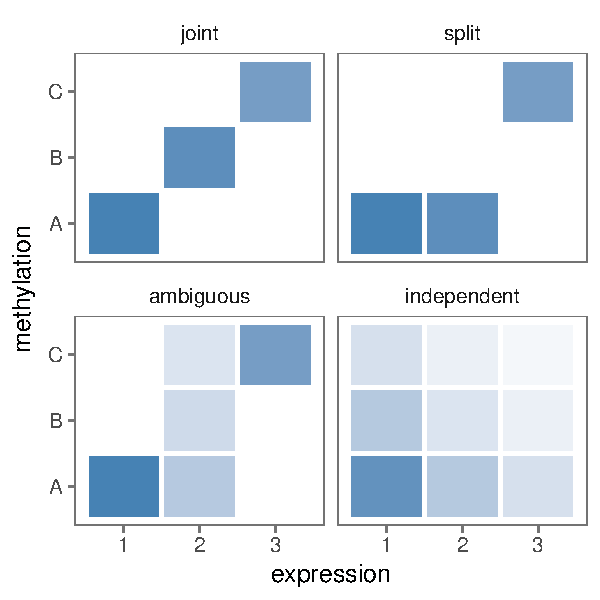
\includegraphics[width=\textwidth]{Figures/cdc-example-pi.pdf}
\end{block}

\end{column}


\begin{column}{.32\linewidth}

\begin{block}{Local vs. global clusters}
  Each context $m$ has \emph{local} mixture weights $\bm{\pi}^{(m)}$:
  \begin{align*}
    \small
    \bm{\pi}^{(m)} &\sim \text{Dirichlet}\left(\frac{\alpha_m}{K^{(m)}}, \dots, \frac{\alpha_m}{K^{(m)}} \right)
  \end{align*}
% \end{block}
% \begin{block}{Global clusters}
  We define the \emph{global} mixture distribution for two contexts as:
  \begin{align*}
    \small
    \bm{\rho} &\sim \text{Dirichlet}\left(\gamma \;
      \text{vec}\left(\bm{\pi}^{(1)} \otimes \bm{\pi}^{(2)}\right)\right) \\
    \begin{split}
      \small
      \bm{\pi}^{(1)} \otimes \bm{\pi}^{(2)} \; &= \;
      \begin{pmatrix}
        \pi^{(1)}_1 \pi_1^{(2)} & \pi^{(1)}_1 \pi_2^{(2)} & \cdots &
        \pi^{(1)}_1 \pi^{(2)}_K \\[0.5em]
        \pi^{(1)}_2 \pi_1^{(2)} & \pi^{(1)}_2 \pi_2^{(2)} & \cdots &
        \pi^{(1)}_2 \pi^{(2)}_K \\[0.5em]
        \vdots  & \vdots  & \ddots & \vdots  \\[0.5em]
        \pi^{(1)}_K \pi^{(2)}_1 & \pi^{(1)}_K \pi^{(2)}_2 & \cdots &
        \pi^{(1)}_K \pi^{(2)}_K
      \end{pmatrix}
      \end{split}
  \end{align*}
  {\small \citejournal{gabasova_clusternomics:_2017-1}}
\end{block}

\begin{block}{Simulated data}
  Two contexts each with two well separated clusters. Simulate 100 data sets
  with $p \sim \textnormal{Uniform}(0, \frac{1}{2})$.
  Sample 100 points with cluster probabilities $(p, 1-p)$ and 100 more with $(1-p, p)$.
  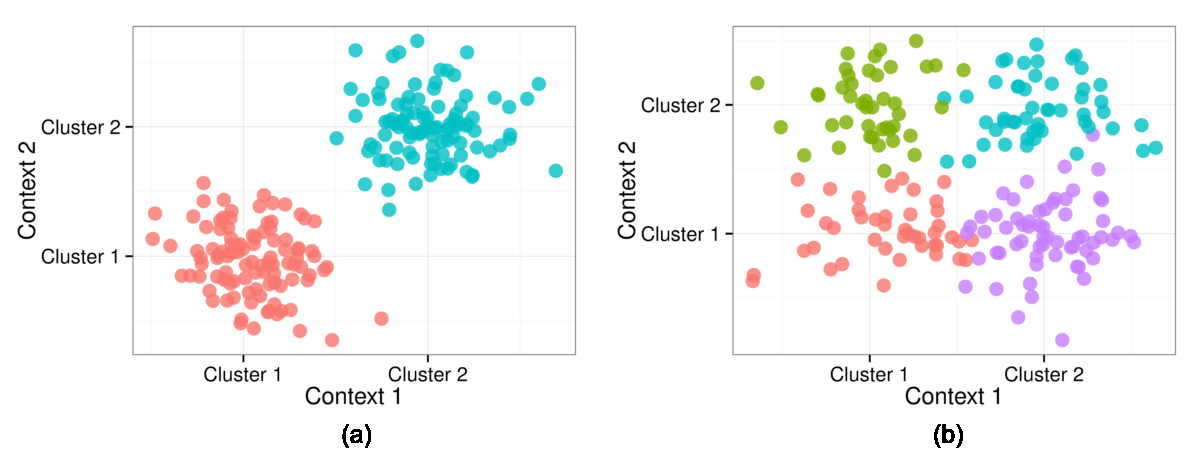
\includegraphics[width=\textwidth]{Figures/simulated-data}
\end{block}

\begin{block}{Simulated data: results}
  % 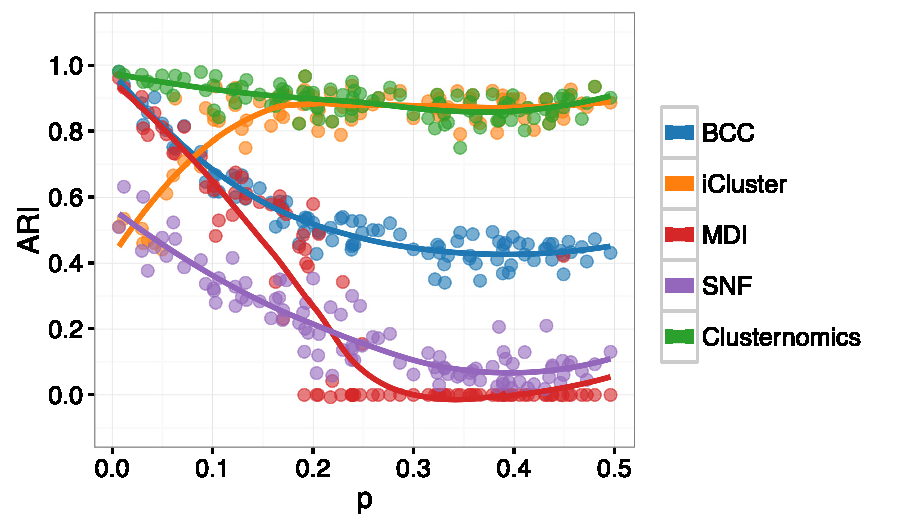
\includegraphics[width=\textwidth]{Figures/simulated-ARI}
% \end{block}

% \begin{block}{Mis-specified number of clusters}
  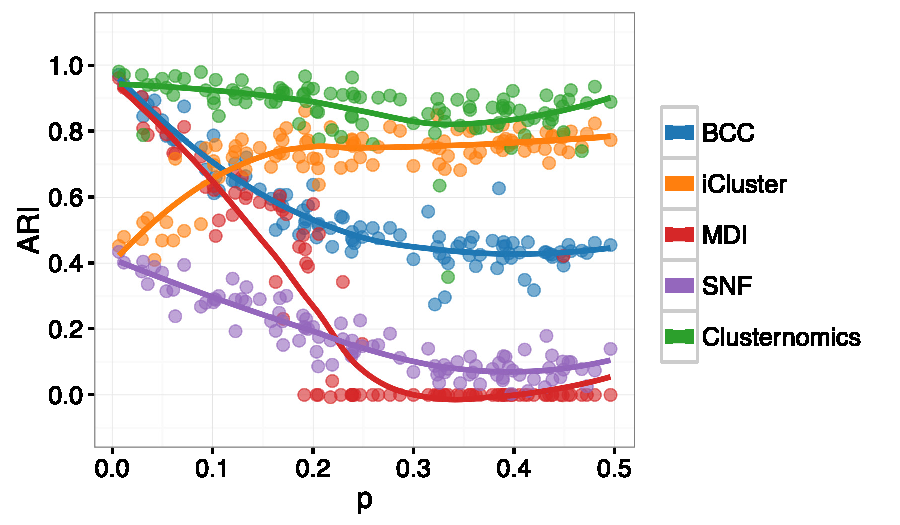
\includegraphics[width=\textwidth]{Figures/simulated-ARI-misspecified}
\end{block}

\begin{block}{Subtypes in breast cancer}
  348 patients diagnosed with breast cancer.
  Four different contexts:
  \begin{enumerate}
    \item RNA gene expression for 645 genes
    \item DNA methylation for 574 probes
    \item expression for 423 microRNAs
    \item reverse-phase protein array (RPPA) for 171 proteins
  \end{itemize}
  Allow 3 local clusters per context and 18 global clusters.
\end{block}

% \begin{block}{Global cluster sizes}
%   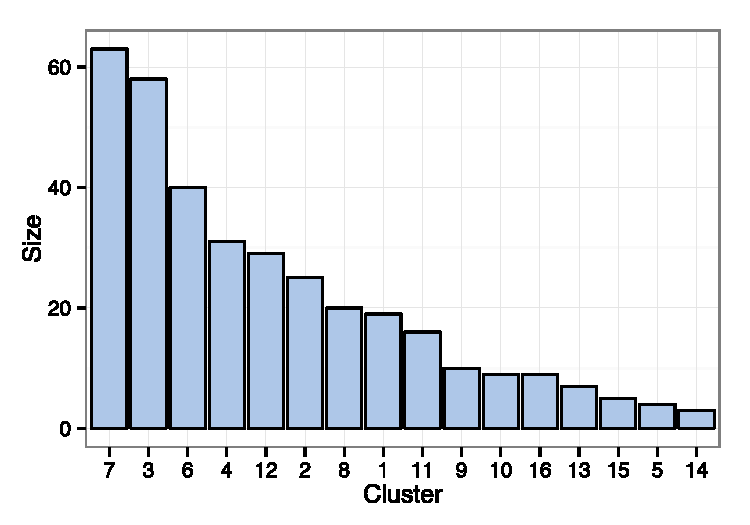
\includegraphics[width=\textwidth]{Figures/breast-sizes}
% \end{block}


\begin{block}{Survival outcomes}
  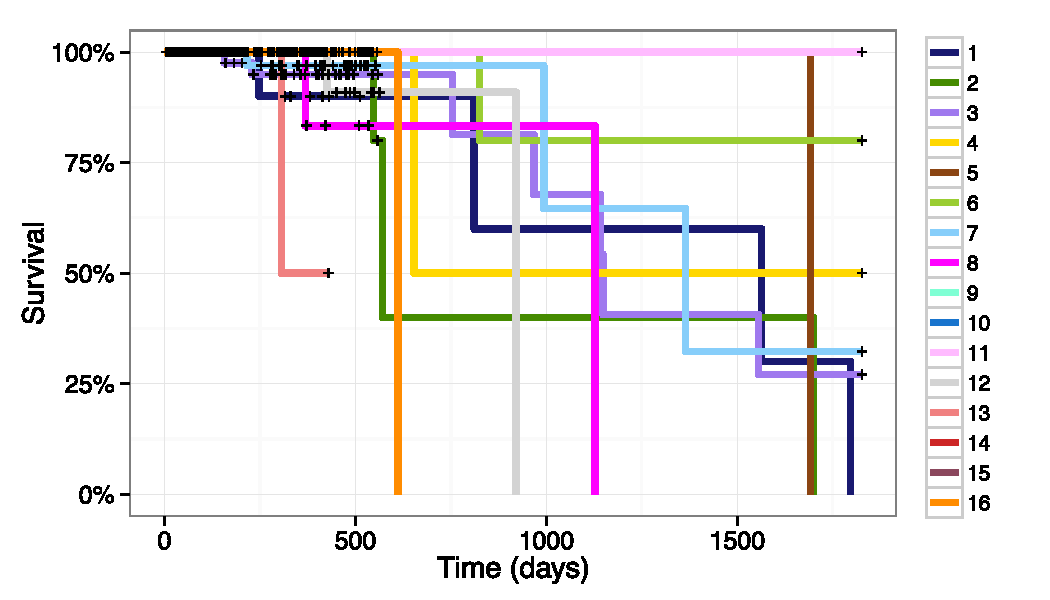
\includegraphics[width=\textwidth]{Figures/breast-survival} \\
  log-rank test $p = 0.038$
\end{block}

\end{column}


\begin{column}{.32\linewidth}

\begin{block}{Local clusters}
  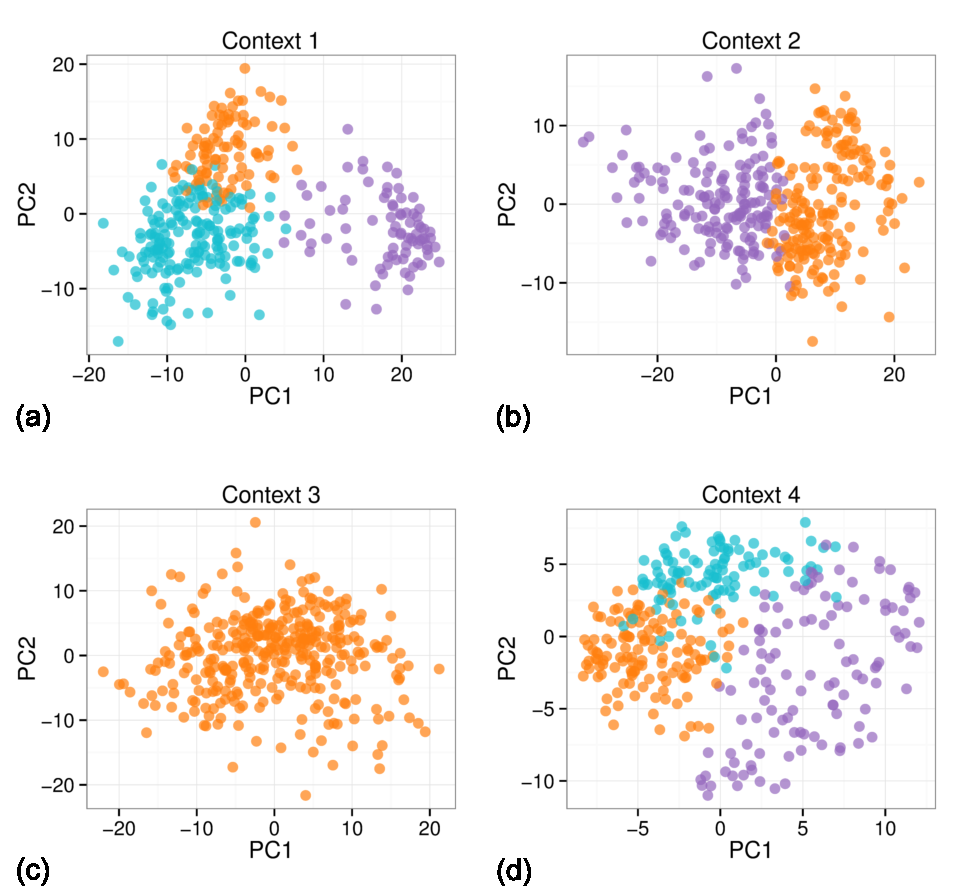
\includegraphics[width=\textwidth]{Figures/breast-PCA-local}
\end{block}

\begin{block}{Global clusters}
  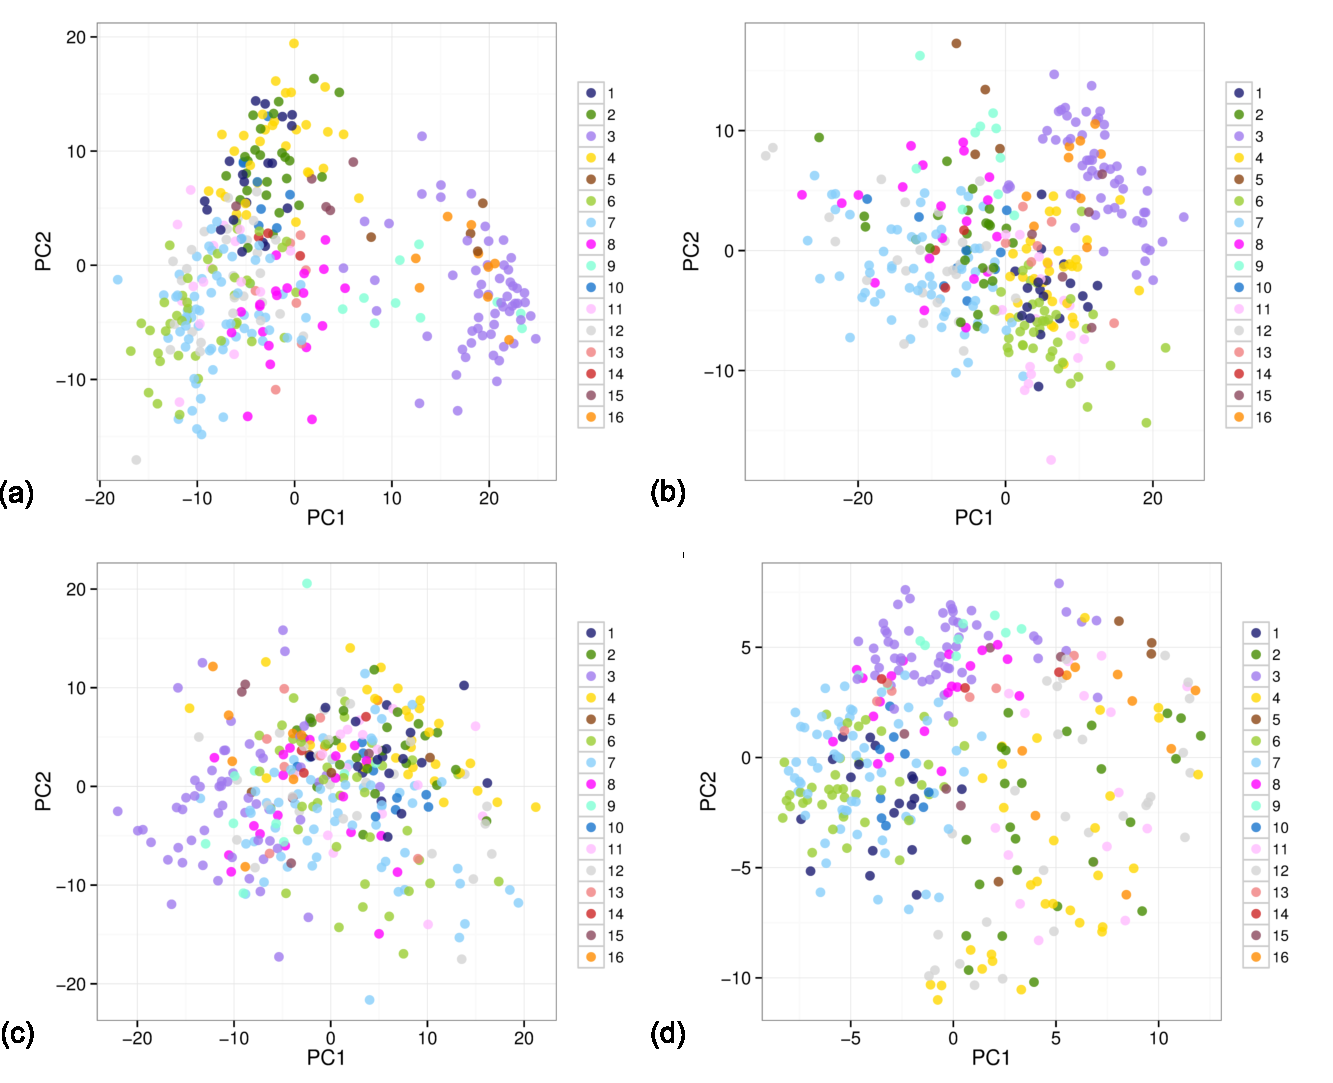
\includegraphics[width=\textwidth]{Figures/breast-PCA}
\end{block}

\begin{block}{Two specific clusters}
  Clusters 1 (dark blue, 19 samples) and 6 (light green, 40 samples)
  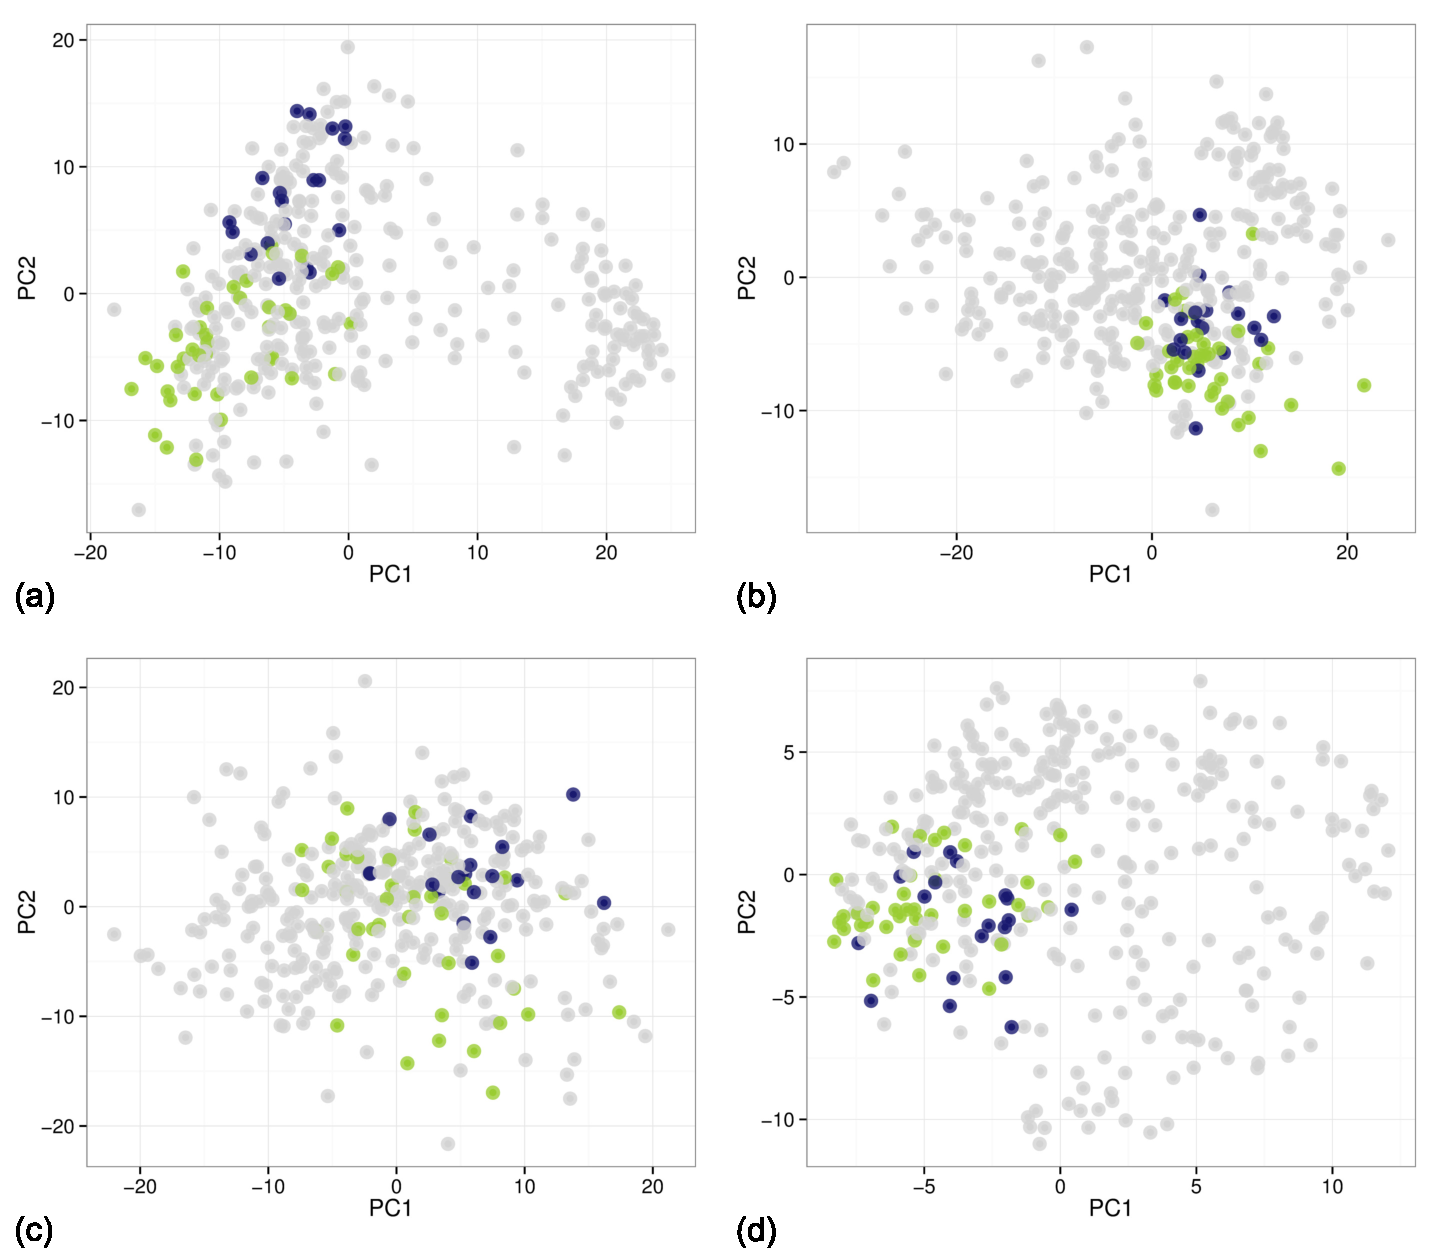
\includegraphics[width=\textwidth]{Figures/breast-PCA-two} \\
  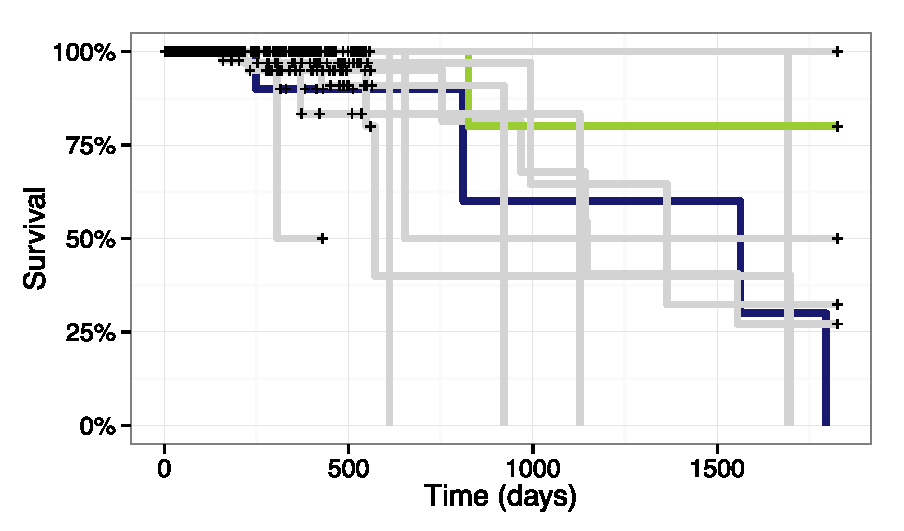
\includegraphics[width=\textwidth]{Figures/breast-survival-two} \\
  log-rank test $p = 0.012$
\end{block}

% \begin{block}{References}
%   % \renewcommand*{\bibfont}{\scriptsize}
%   \renewcommand*{\bibfont}{\footnotesize}
%   \printbibliography
% \end{block}

\end{column}
\end{columns}

\end{frame}
\end{document}
